\section{Sensibilidad}\label{sec:sensibilidad}

La sensibilidad S1 estudia seis variantes de X0 que cambian un solo factor:
aforo $\pm$10~\%, velocidad de marcha $\pm$15~\% o tiempo de servicio en el torno
$\pm$25~\%. El resto de parámetros es el del escenario base, con salida ordinaria
y sin alarma. Las variaciones no tienen el mismo tamaño entre factores, así que
las diferencias no son una clasificación universal de su importancia, y no se
exploran combinaciones de factores.

\begin{table}[htbp]
\centering\small
\caption{Diferencias emparejadas variante $-$ X0 (min), con IC del 95~\%.}
\label{tab:s1}
\begin{tabular}{@{}lrrrr@{}}
\toprule
Variante & Parejas & Espera media & Tiempo de acceso & Vaciado ordinario \\
\midrule
Aforo $-$10~\% & 180 & $-$0,1036 $\pm$ 0,0050 & $-$0,1085 $\pm$ 0,0051 & $-$0,6734 $\pm$ 0,0342 \\
Aforo $+$10~\% & 73 & $+$0,2867 $\pm$ 0,0114 & $+$0,2924 $\pm$ 0,0112 & $+$0,7604 $\pm$ 0,0228 \\
Velocidad $-$15~\% & 180 & 0 & $+$0,2748 $\pm$ 0,0001 & $+$0,3658 $\pm$ 0,0532 \\
Velocidad $+$15~\% & 180 & 0 & $-$0,1983 $\pm$ 0,0001 & $-$0,0861 $\pm$ 0,0182 \\
Servicio $-$25~\% & 180 & $-$0,1613 $\pm$ 0,0069 & $-$0,1772 $\pm$ 0,0069 & $\approx$ 0 \\
Servicio $+$25~\% & 30 & $+$1,2172 $\pm$ 0,0341 & $+$1,2283 $\pm$ 0,0339 & $\approx$ 0 \\
\bottomrule
\end{tabular}
\end{table}

% La figura S1 tiene tres paneles en una sola imagen; se recortan con trim/clip
% (unidades: bp sobre la imagen de 4590 x 1440 px a 300 ppp) para mostrarlos más
% grandes. No se modifica la imagen ni sus datos.
\begin{figure}[p]
\centering
\begin{subfigure}{\textwidth}\centering
  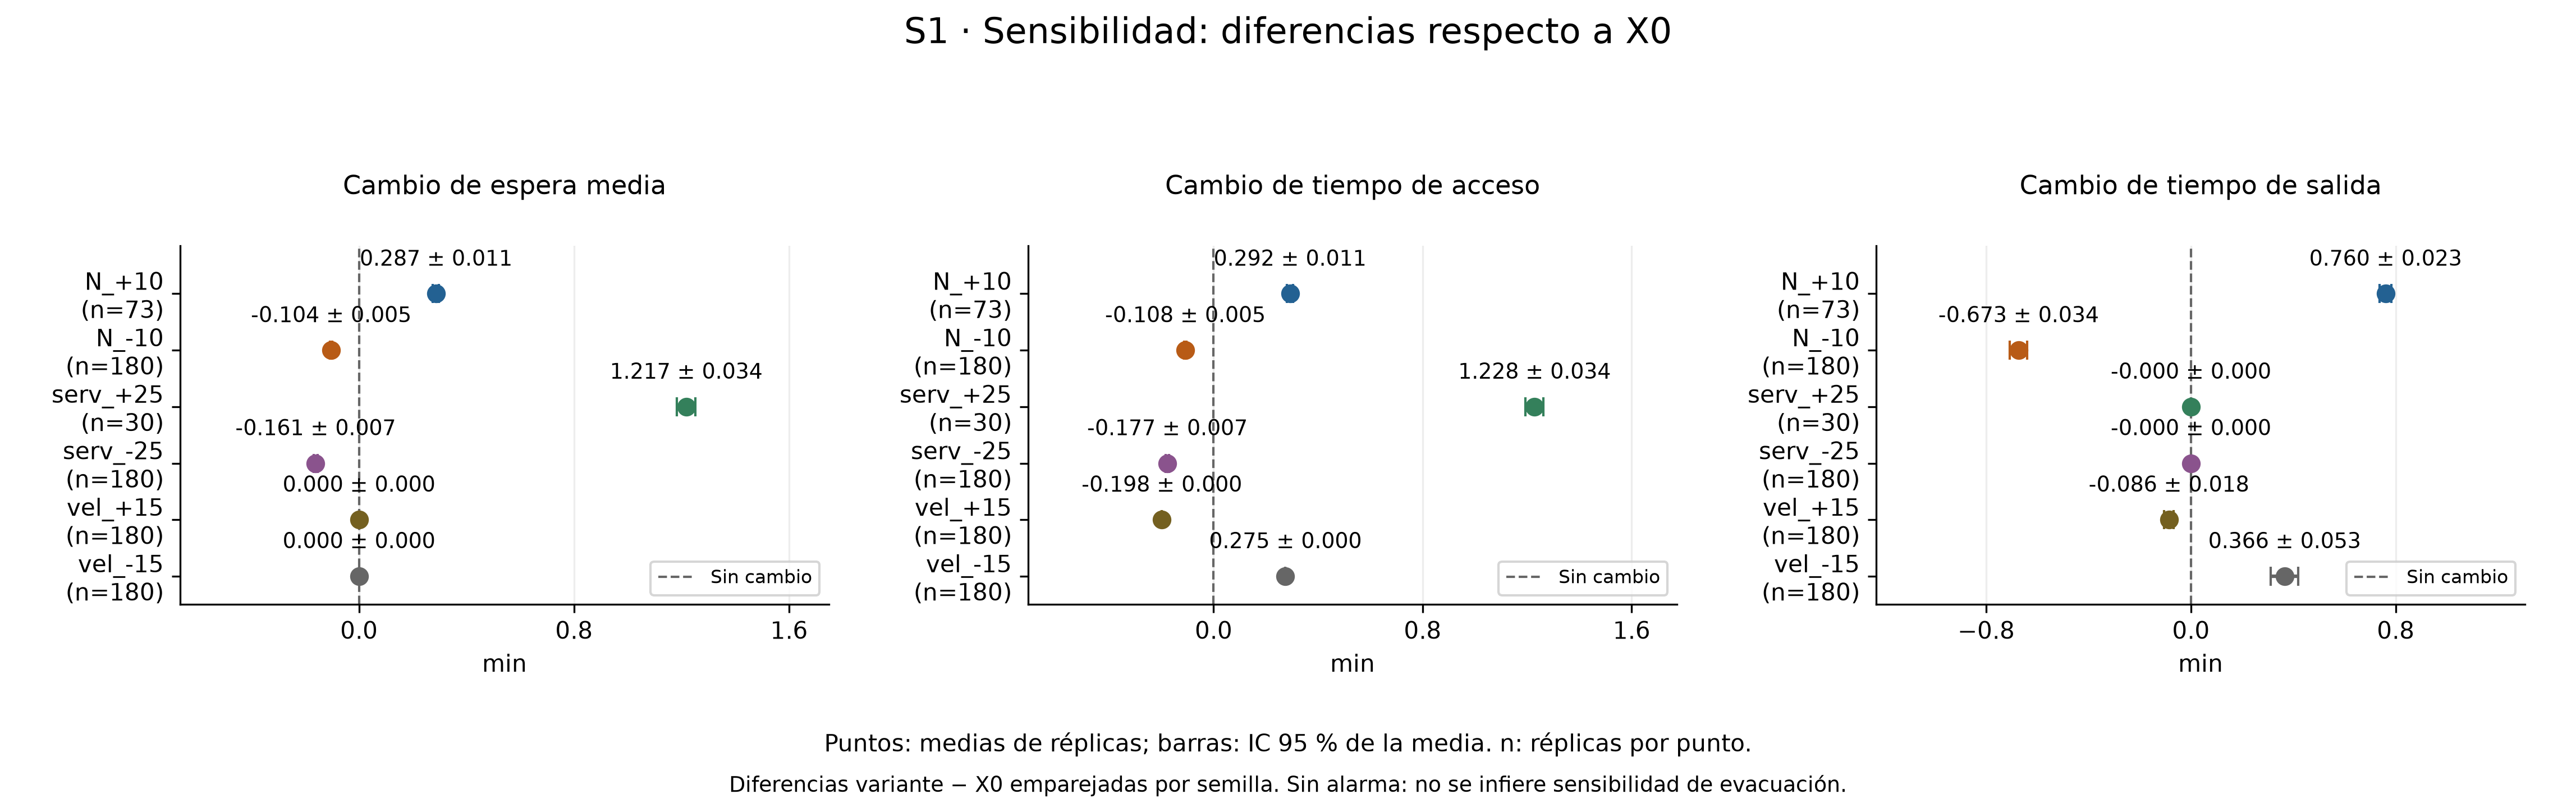
\includegraphics[width=0.66\textwidth,trim=0 57.6 732 72,clip]{S1.png}
  \caption{Cambio de la espera media.}
\end{subfigure}\\[0.6em]
\begin{subfigure}{\textwidth}\centering
  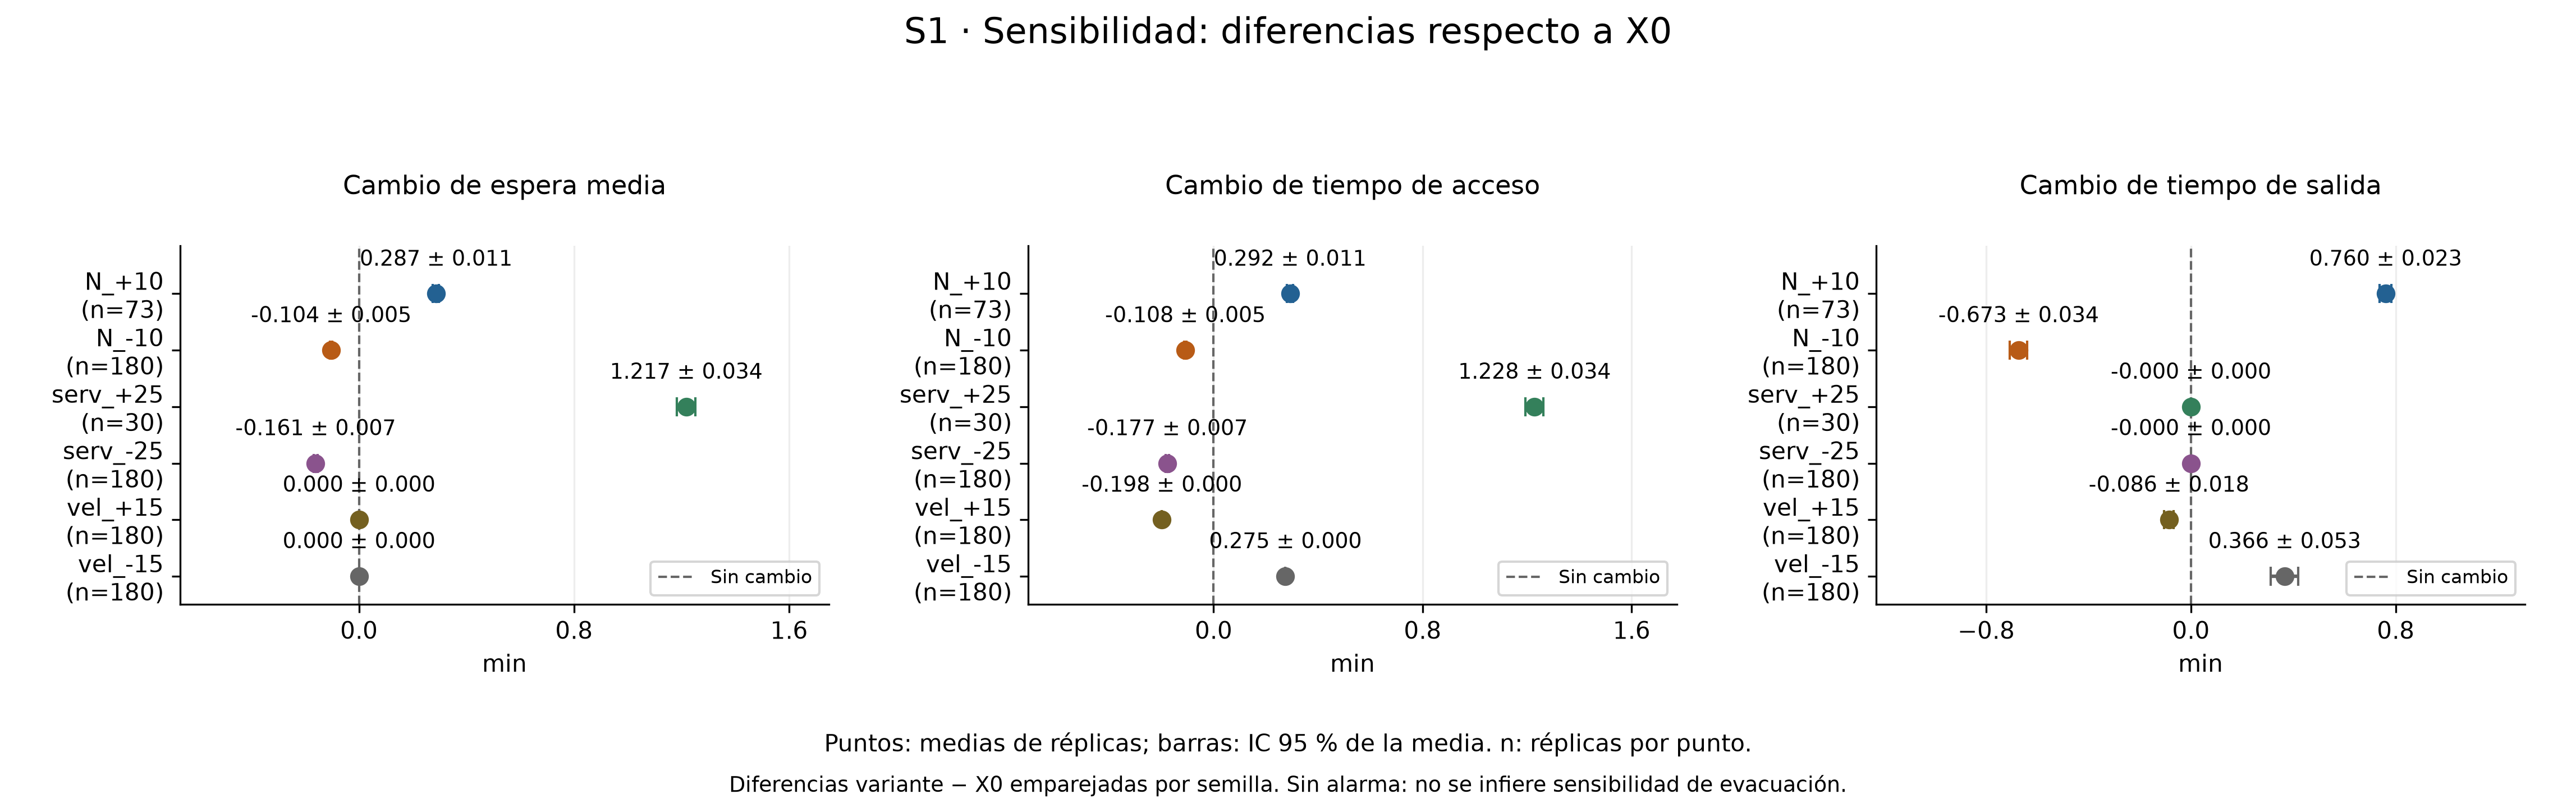
\includegraphics[width=0.66\textwidth,trim=369.6 57.6 369.6 72,clip]{S1.png}
  \caption{Cambio del tiempo de acceso.}
\end{subfigure}\\[0.6em]
\begin{subfigure}{\textwidth}\centering
  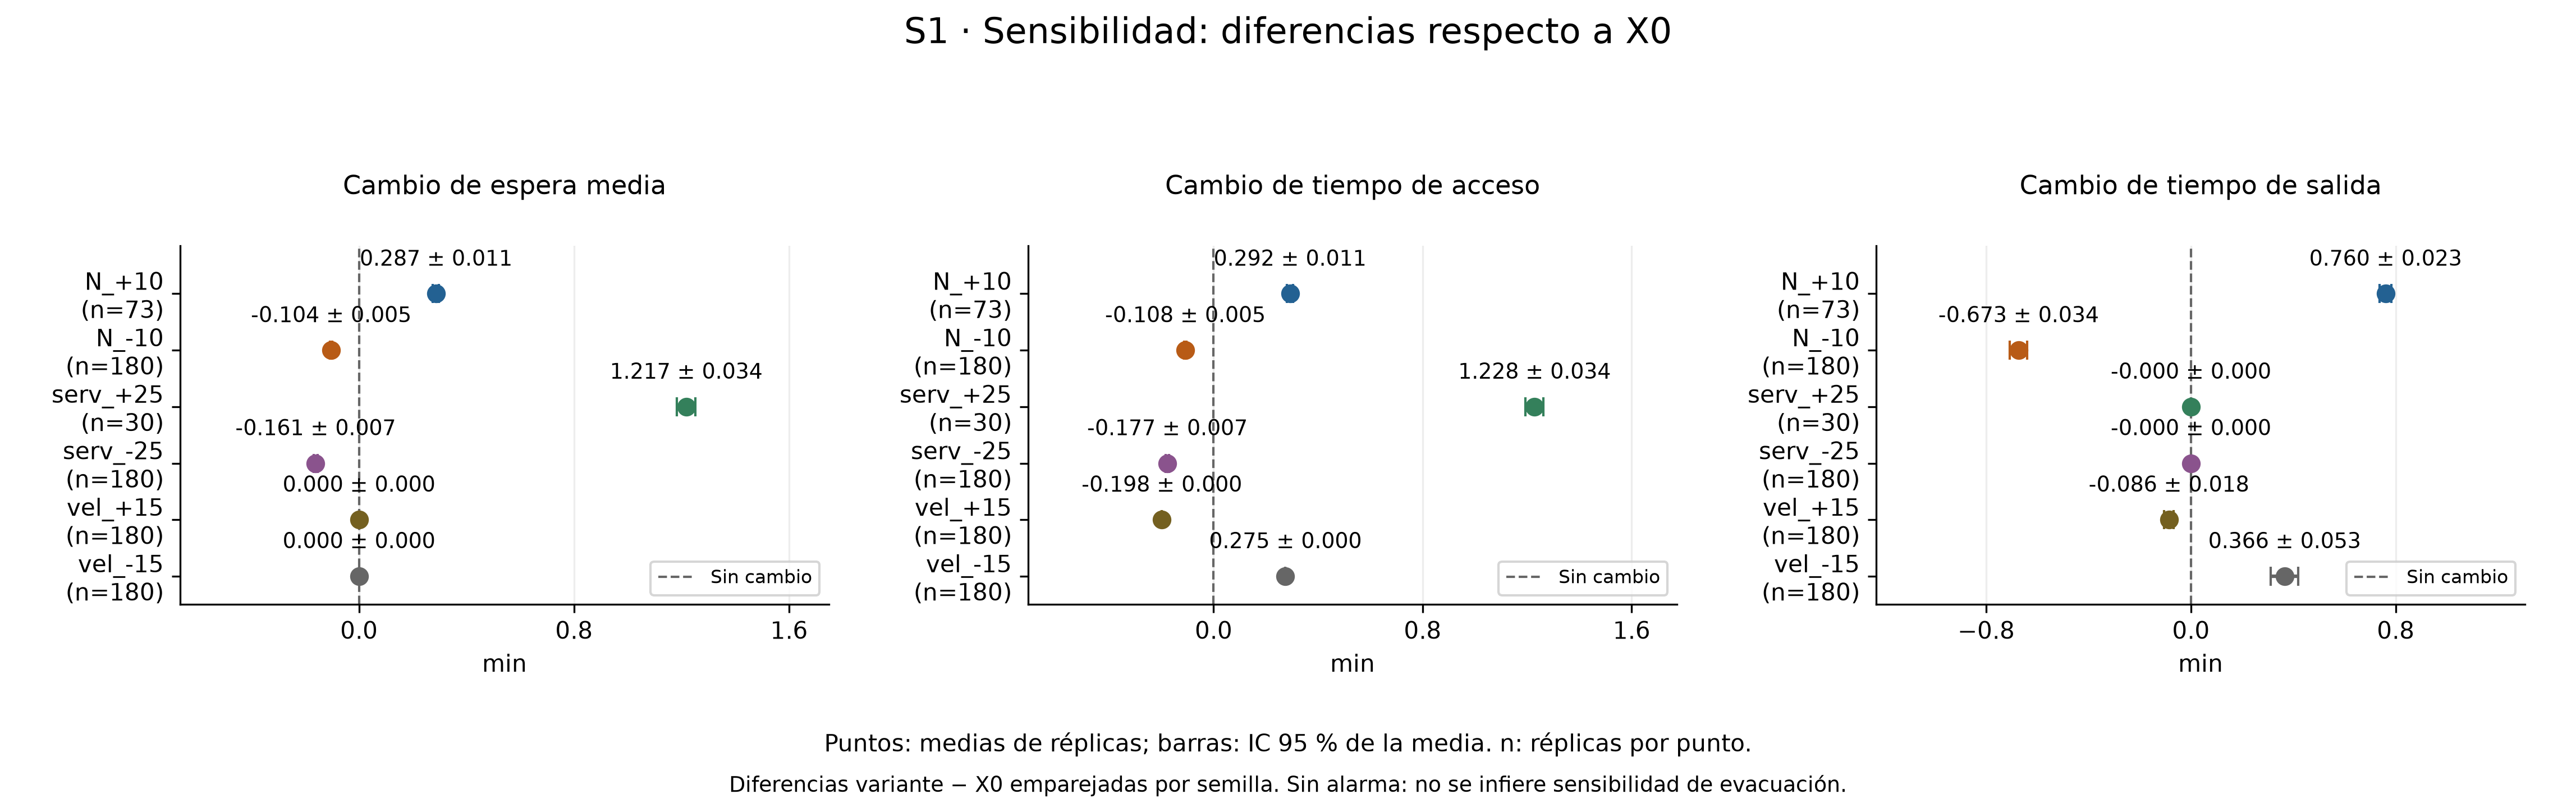
\includegraphics[width=0.66\textwidth,trim=732 57.6 0 72,clip]{S1.png}
  \caption{Cambio del tiempo de vaciado ordinario.}
\end{subfigure}
\caption{S1. Cambio respecto a X0 en cada variante (N: aforo; serv: tiempo de
servicio; vel: velocidad), emparejado por semilla. Puntos: medias; barras: IC
del 95~\%; $n$: parejas por variante (entre 30 y 180). Las variantes no tienen
alarma, así que no indican la sensibilidad de la evacuación.}
\label{fig:s1}
\end{figure}

\textbf{Aforo.} Reducir el público un 10~\% baja la espera media unos 0,104~min;
aumentarlo un 10~\% la sube unos 0,287~min. El efecto no es simétrico porque el
escenario base ya está cerca de la capacidad de entrada en la punta
($\rho=0{,}93$, y 1,02 con un 10~\% más). También cambia el vaciado, porque
cruzan las salidas más o menos personas.

\textbf{Servicio.} Un 25~\% más de tiempo de control sube la espera media unos
1,217~min (unos 73~s) frente a una base de 0,192~min; un 25~\% menos la baja
unos 0,161~min, porque la espera no puede ser negativa. La respuesta a P2 es, por
tanto, sensible al tiempo de servicio supuesto, aunque con 3 tornos el objetivo
se sigue cumpliendo (P2). El vaciado apenas cambia: la entrada termina mucho
antes del final del partido.

\textbf{Velocidad.} No cambia la cola de entrada, que es idéntica semilla a
semilla, porque la marcha ocurre después del control y el modelo no transmite
bloqueos del interior hacia el torno. Sí cambian el acceso y la salida, que
incluyen desplazamientos: la lentitud aumenta el acceso unos 0,275~min y el
aumento de velocidad lo reduce unos 0,198~min, coherente con que el tiempo de
recorrido depende del inverso de la velocidad.

\textbf{Alcance.} S1 permite valorar si algunas conclusiones dependen mucho de
los parámetros inciertos ensayados. No es una calibración con datos reales ni
demuestra robustez frente a cualquier cambio: los IC pequeños solo indican poca
incertidumbre muestral bajo las hipótesis del modelo. Estas variantes no tienen
alarma, así que no son una sensibilidad de la evacuación.
